% Provenance (never printed): see sources/outline_sources.md (Year 1: heat sources,
% radiogenic and secular cooling; heat-flow measurement; the steady conductive geotherm
% with heat production; convection against conduction; the lithosphere as a thermal
% boundary layer). Curves from figdata/bachelor-1/geotherms.py; exercise and problem
% values in the Book 3 scratch calculator calc/ch10.py.
\chapter{पृथ्वी का ऊष्मा-बजट}\label{ch:b1:heat-budget}

जापानी आल्प्स में एक पहाड़ के नीचे, एक पुरानी खदान की गुफ़ा में, एक हज़ार टन द्रव सिंटिलेटर से भरा एक टैंक प्रकाश की मद्धम चमकों की प्रतीक्षा करता है। अधिकांश चमकें उसके आसपास के देश के परमाणु रिएक्टरों में बनने वाले प्रति-न्यूट्रिनो से आती हैं, पर कुछ नीचे से आती हैं: पृथ्वी के भीतर का यूरेनियम और थोरियम अपने क्षय के समय प्रति-न्यूट्रिनो उत्सर्जित करते हैं, और ये पूरे ग्रह को ऐसे पार करते हैं मानो वह खाली हो। 2135 दिनों की गिनती में डिटेक्टर ने 841 संभावित घटनाएँ दर्ज कीं, जिनमें से 106 पृथ्वी के भीतर से मानी गईं। इन मुट्ठी भर चमकों से, 2011 में उसकी टीम ने अनुमान लगाया कि यूरेनियम और थोरियम का क्षय पृथ्वी को लगभग 20 टेरावाट से गरम करता है। पूरा ग्रह लगभग 47 खोता है। यह अध्याय उस अंतर का लेखा-जोखा देता है: पृथ्वी की ऊष्मा कहाँ से आती है, उससे बाहर बहती ऊष्मा कैसे मापी जाती है, जब ऊष्मा चालन से ले जाई जाती है तब तापमान गहराई के साथ कैसे बढ़ता है, \omterm{def:b1:layered-earth:layers}{प्रावार} को संवहन क्यों करना पड़ता है, और प्लेटें उस संवहन की ठंडी ऊपरी सीमा क्यों हैं।

\begin{recall}
ऊष्मा गरम से ठंडे की ओर बहती है; किसी चट्टान की ऊष्मीय चालकता $k$ बताती है कि ऊष्मा उसे कितनी आसानी से पार करती है, और उसकी ऊष्मीय विसरणशीलता $\kappa = k/(\rho c)$ बताती है कि तापमान-परिवर्तन कितनी तेज़ी से फैलता है (भौतिकी, विश्वविद्यालय वर्ष 2)। रेडियोधर्मी नाभिक एक निश्चित अर्ध-आयु से क्षय होते हैं (भौतिकी)। \omterm{def:b1:heat-budget:geotherm}{जियोथर्म} के साथ गहराई पर तापमान बढ़ता है, और \omterm{def:b1:layered-earth:layers}{प्रावार} संवहन करता है (पुस्तक 2, कक्षा 11 और 12)। \omterm{def:b1:layered-earth:lithosphere}{स्थलमंडल} पृथ्वी का सुदृढ़ बाहरी कवच है (\cref{ch:b1:layered-earth})।
\end{recall}

\section{ऊष्मा कहाँ से आती है}

\begin{definition}[ऊष्मा-प्रवाह]
\label{def:b1:heat-budget:heat-flow}
\emph{ऊष्मा-प्रवाह}\index{ऊष्मा-प्रवाह} $q$ पृथ्वी की सतह के एक बिंदु पर, या सतही ऊष्मा-प्रवाह-घनत्व, वह आंतरिक मूल की शक्ति है जो वहाँ इकाई क्षेत्रफल से होकर बाहर की ओर पार होती है, बाहर की दिशा को धनात्मक गिनते हुए। इसे \unit{W.m^{-2}} में मापा जाता है, व्यवहार में \unit{mW.m^{-2}} में। पूरी सतह पर समाकलित करने पर यह पृथ्वी की ऊष्मा-हानि $Q = \oint q\,\mathrm dS$ देता है।
\end{definition}

\omterm{def:b1:heat-budget:heat-flow}{ऊष्मा-प्रवाह} दसियों हज़ार स्थानों पर मापा गया है। 2010 में प्रकाशित \num{38347} मापों के एक संकलन से नीचे के औसत मान मिलते हैं, जिसमें महासागर और महाद्वीप अलग-अलग गिने गए हैं:
\begin{center}
\small
% ledger: dd10:split, dd10:total
\begin{tabular}{lccc}
\hline
 & क्षेत्रफल (\unit{m^2}) & ऊष्मा-हानि (\unit{TW}) & औसत \omterm{def:b1:heat-budget:heat-flow}{ऊष्मा-प्रवाह} (\unit{mW.m^{-2}}) \\
\hline
महाद्वीप & \num{2.073e14} & 14.7 & 70.9 \\
महासागर & \num{3.028e14} & 31.9 & 105.4 \\
पूरी पृथ्वी & \num{5.101e14} & 46.7 & 91.6 \\
\hline
\end{tabular}
\end{center}
कुल, अपनी अनिश्चितता तक पूर्णांकित, $Q = \qty[uncertainty-mode=separate]{47 \pm 2}{TW}$ है। इसका दो-तिहाई भाग समुद्र-तल से निकलता है, जो महाद्वीपों से युवा और पतला है। यह एक छोटा प्रवाह है: सूर्य पृथ्वी को लगभग \qty{173000}{TW} देता है, और आंतरिक ऊष्मा सतह पर ऊर्जा-बजट का \qty{0.03}{\percent} है। % ledger: nasa:solar-mean
लेकिन यही वह प्रवाह है जो ज्वालामुखियों, प्लेटों और पर्वत-निर्माण को चलाता है, और इसके दो स्रोत हैं।

\begin{definition}[रेडियोजनिक ऊष्मा-उत्पादन]
\label{def:b1:heat-budget:heat-production}
\emph{रेडियोजनिक ऊष्मा-उत्पादन}\index{रेडियोजनिक ऊष्मा-उत्पादन} $A$ किसी चट्टान का वह ऊष्मा है जो उसमें मौजूद रेडियोधर्मी नाभिकों के क्षय से प्रति इकाई आयतन और प्रति इकाई समय मुक्त होती है, \unit{W.m^{-3}} में, व्यवहार में \unit{\micro W.m^{-3}} में। घनत्व $\rho$ वाली और ऊष्मा-उत्पादक तत्वों के द्रव्यमान-अंश $C_i$ रखने वाली एक चट्टान, जिनमें से हर एक प्रति किलोग्राम तत्व $H_i$ वाट मुक्त करता है, की
\[
  A = \rho \sum_i C_i H_i .
\]
\end{definition}

इस ऊष्मा का लगभग सारा भाग चार समस्थानिक उत्पन्न करते हैं, क्योंकि वे दीर्घजीवी, पर्याप्त प्रचुर और ऊर्जावान हैं: \ce{^{238}U}, \ce{^{235}U}, \ce{^{232}Th} और \ce{^{40}K}। प्रति किलोग्राम हर तत्व की ऊष्मा, उसके रेडियोधर्मी समस्थानिक की प्रति किलोग्राम ऊष्मा को उस समस्थानिक के तत्व में अंश (परमाणुओं में) से गुणा करने पर मिलती है (\cref{exo:b1:heat-budget:3}):
\begin{center}
\small
% ledger: dye:isotope-heat, iaea:isotopes
\begin{tabular}{lcccc}
\hline
समस्थानिक & अर्ध-आयु & समस्थानिक की प्रति किलोग्राम ऊष्मा & तत्व में अंश (परमाणु) & तत्व की प्रति किलोग्राम ऊष्मा \\
 & (\unit{Gyr}) & (\unit{W.kg^{-1}}) & तत्व में (परमाणु) & (\unit{W.kg^{-1}}) \\
\hline
\ce{^{238}U} & 4.468 & \num{9.513e-5} & \qty{99.274}{\percent} & U: \num{9.85e-5} \\
\ce{^{235}U} & 0.704 & \num{5.685e-4} & \qty{0.720}{\percent} & \\
\ce{^{232}Th} & 14.0 & \num{2.628e-5} & लगभग सभी & Th: \num{2.63e-5} \\
\ce{^{40}K} & 1.248 & \num{2.847e-5} & \qty{0.0117}{\percent} & K: \num{3.40e-9} \\
\hline
\end{tabular}
\end{center}
पोटैशियम प्रति किलोग्राम यूरेनियम से तीस हज़ार गुना कम ऊष्मा मुक्त करता है, पर वह कई चट्टानों का एक प्रमुख तत्व है, जो प्रतिशत में गिना जाता है, जबकि यूरेनियम और थोरियम दस लाख भागों में गिने जाते हैं। तीनों से समृद्ध चट्टानें ग्रेनाइट और उनके संबंधी हैं; सबसे निर्धन \omterm{def:b1:layered-earth:layers}{प्रावार} के पेरिडोटाइट हैं। \num{2188} विश्लेषणों के एक संकलन से ये माध्यिकाएँ मिलती हैं, \unit{\micro
W.m^{-3}} में:
\begin{center}
\small
% ledger: vila:heat-production
\begin{tabular}{lclclc}
\hline
राइओलाइट & 2.55 & पंक-शैल & 1.44 & गैब्रो & 0.35 \\
ग्रेनाइट & 2.43 & बलुआ पत्थर & 0.82 & बेसाल्ट & 0.21 \\
ग्रैनोडायोराइट & 1.88 & कार्बोनेट चट्टानें & 0.42 & अति-मैफ़िक चट्टानें & 0.11 \\
\hline
\end{tabular}
\end{center}
हर समूह के भीतर का प्रसार विस्तृत है: ग्रेनाइट का एक-चौथाई, जिसकी दर \qty{1.74}{\micro W.m^{-3}} से कम उत्पन्न करता है, एक-चौथाई \qty{3.23}{\micro W.m^{-3}} से अधिक। महाद्वीपीय \omterm{def:b1:layered-earth:layers}{भूपर्पटी} इन तत्वों से समृद्ध है, महासागरीय \omterm{def:b1:layered-earth:layers}{भूपर्पटी} और \omterm{def:b1:layered-earth:layers}{प्रावार} निर्धन; पर \omterm{def:b1:layered-earth:layers}{प्रावार} इतना बड़ा है कि वह अब भी ग्रह के ऊष्मा-स्रोतों का एक बड़ा भाग रखता है।

\begin{definition}[दीर्घकालिक शीतलन]\label{def:b1:heat-budget:secular-cooling}
\emph{दीर्घकालिक शीतलन}\index{दीर्घकालिक शीतलन} पृथ्वी की ऊष्मा-हानि का वह भाग है जो उसके आंतरिक भाग, \omterm{def:b1:layered-earth:layers}{प्रावार} और कोर के तापमान में धीमी कमी से मिलता है: ग्रह के बनने के बाद से संचित ऊष्मा का मुक्त होना, भंडारों के लिए $-\sum_j M_j c_j\,\mathrm dT_j/\mathrm dt$ की दर से, जहाँ $M_j$ द्रव्यमान, $c_j$ विशिष्ट ऊष्मा और $T_j$ औसत तापमान है।
\end{definition}

ऊर्जा संरक्षण पूरे पृथ्वी का बजट देता है: सतह पर खोई गई ऊष्मा रेडियोजनिक उत्पादन और \omterm{def:b1:heat-budget:secular-cooling}{दीर्घकालिक शीतलन} का योग है,
\[
  Q = H_{\text{rad}} + Q_{\text{sc}} .
\]
पहले पद का एक भाग जियोन्यूट्रिनो मापते हैं: 2011 का परिणाम, जिसने दो डिटेक्टरों को मिलाया, यूरेनियम और थोरियम को \qty{20}{TW} श्रेय देता है, और \ce{^{40}K}, जिसके प्रति-न्यूट्रिनो उस तरीके से पहचाने जाने के लिए बहुत दुर्बल हैं, लगभग \qty{4}{TW} जोड़ने के लिए जाना जाता है।
% ledger: kamland:2011
अतः ऊष्मा-हानि का लगभग आधा भाग रेडियोजनिक है, और दूसरा आधा, लगभग \qty{23}{TW}, \omterm{def:b1:heat-budget:secular-cooling}{दीर्घकालिक शीतलन} है। उस शीतलन का एक भाग कोर का है: \omterm{def:b1:layered-earth:discontinuity}{कोर–प्रावार सीमा} के आरपार बहने वाली ऊष्मा का अनुमान \qtyrange{5}{15}{TW} है। ये आँकड़े अनिश्चित हैं: माप स्वयं लगभग \qty{9}{TW} की अनिश्चितता रखता है, और अब तक के जियोन्यूट्रिनो परिणाम रेडियोजनिक भाग को केवल \qtyrange{15}{41}{TW} में सीमित करते हैं, जबकि पृथ्वी के विभिन्न प्रकार के मॉडल \qtyrange{14}{46}{TW} तक फैलते हैं। सतह पर मापा गया कुल बजट का सबसे सुज्ञात पद है (नीचे का चित्र)।
% ledger: dye:radiogenic

\begin{omfigure}
\begin{tikzpicture}[x=0.24cm, y=1cm, font=\small]
% ledger: dd10:split, kamland:2011, dye:radiogenic
% losses
\fill[blue!22] (0,1.6) rectangle (31.9,2.3);
\fill[brown!35] (31.9,1.6) rectangle (46.6,2.3);
\draw (0,1.6) rectangle (46.6,2.3);
\draw (31.9,1.6) -- (31.9,2.3);
\node at (15.95,1.95) {महासागर 31.9};
\node at (39.25,1.95) {महाद्वीप 14.7};
\node[anchor=east, align=right, font=\small] at (-0.5,1.95) {सतह पर\\खोई गई};
% sources
\fill[orange!35] (0,0) rectangle (20,0.7);
\fill[yellow!45] (20,0) rectangle (24,0.7);
\fill[red!18] (24,0) rectangle (46.7,0.7);
\draw (0,0) rectangle (46.7,0.7);
\draw (20,0) -- (20,0.7) (24,0) -- (24,0.7);
\node at (10,0.35) {U और Th 20};
\node at (22,0.35) {K 4};
\node at (35.35,0.35) {दीर्घकालिक शीतलन $\approx 23$};
\node[anchor=east, align=right] at (-0.5,0.35) {स्रोत};
% core part of secular cooling (range)
\draw[red!60!black, very thick] (24,-0.25) -- (29,-0.25);
\draw[red!60!black, thick, densely dashed] (29,-0.25) -- (39,-0.25);
\draw[red!60!black] (24,-0.15) -- (24,-0.35) (39,-0.15) -- (39,-0.35);
\node[anchor=north, font=\scriptsize, red!60!black] at (31.5,-0.3) {कोर–प्रावार सीमा के आरपार ऊष्मा, \qtyrange{5}{15}{TW}};
% radiogenic range
\draw[|-|, orange!70!black, thick] (15,1.0) -- (41,1.0);
\node[anchor=south, font=\scriptsize, orange!70!black] at (28,1.02) {रेडियोजनिक अनुमानों की परास, \qtyrange{15}{41}{TW}};
% axis
\draw[->] (0,-1.05) -- (50,-1.05) node[right] {TW};
\foreach \x in {0,10,20,30,40} {\draw (\x,-1.0) -- (\x,-1.1) node[below, font=\scriptsize] {\x};}
\end{tikzpicture}

\par\smallskip{\small पृथ्वी का ऊष्मा-बजट। ऊपर: महासागर-तल और महाद्वीपों से खोई गई ऊष्मा, कुल \qty[uncertainty-mode=separate]{47 \pm 2}{TW}। नीचे: उसके स्रोत, जिनमें यूरेनियम और थोरियम का रेडियोजनिक भाग जियोन्यूट्रिनो से मापा गया है और पोटैशियम का अनुमान लगाया गया है; शेष, अंतर से, \omterm{def:b1:heat-budget:secular-cooling}{दीर्घकालिक शीतलन} है, जिसका एक कम ज्ञात भाग कोर देता है। नारंगी पट्टी जियोन्यूट्रिनो मापों द्वारा अनुमत रेडियोजनिक भाग की परास दिखाती है।}
\label{fig:b1:heat-budget:budget}
\end{omfigure}

अतीत में रेडियोजनिक ऊष्मा बड़ी थी, क्योंकि समस्थानिक अधिक प्रचुर थे: \ce{^{235}U} और \ce{^{40}K}, जो अल्पजीवी हैं, तब कहीं अधिक योगदान देते थे (पुस्तक 2, कक्षा 12)। पृथ्वी का ऊष्मीय इंजन दोनों कारणों से धीरे-धीरे ठंडा हो रहा है।

\section{ऊष्मा-प्रवाह का मापन}

\omterm{def:b1:heat-budget:heat-flow}{ऊष्मा-प्रवाह} सीधे नहीं मापा जाता: वह एक तापमान-प्रवणता और एक चालकता से परिकलित होता है।

\begin{proposition}[फ़ूरिये का नियम]\label{prop:b1:heat-budget:fourier}
किसी ऊष्मीय चालकता $k$ वाले माध्यम में ऊष्मा, प्रति इकाई क्षेत्रफल, तापमान-प्रवणता के नीचे उसके समानुपाती दर से चालन द्वारा बहती है। $z$ गहराई हो, नीचे की ओर धनात्मक गिनी गई, और $q$ ऊपर की ओर धनात्मक गिना गया,
\[
  q = k\,\frac{\mathrm dT}{\mathrm dz} .
\]
\end{proposition}
\admitted

यह नियम भौतिकी की पुस्तकों के विश्वविद्यालय वर्ष 2 खंड में स्थापित है। अधिकांश चट्टानें \qtyrange{1.5}{3}{W.m^{-1}.K^{-1}} से लेकर \qty{200}{\celsius} तक ऊष्मा का संचालन करती हैं, गरम होने पर कम; महाद्वीपीय \omterm{def:b1:heat-budget:heat-flow}{ऊष्मा-प्रवाह} के मॉडल ऊपरी \omterm{def:b1:layered-earth:layers}{भूपर्पटी} के ग्रेनाइटी भाग को लगभग \qty{2.7}{W.m^{-1}.K^{-1}} देते हैं;
% ledger: delaney:conductivity, roy:granitic-k
उसमें \qty{25}{K.km^{-1}} की प्रवणता का अर्थ है लगभग \qty{70}{mW.m^{-2}} का \omterm{def:b1:heat-budget:heat-flow}{ऊष्मा-प्रवाह}।

जब किसी बोरहोल के आर-पार की चट्टानों की चालकताएँ भिन्न होती हैं, तो प्रवणता एक से दूसरी में बदलती है, पर \omterm{def:b1:heat-budget:heat-flow}{ऊष्मा-प्रवाह} नहीं बदलता, जब तक उनके बीच ऊष्मा उत्पन्न या संचित न हो। नीचे का प्रस्ताव इसे एक परीक्षण में बदल देता है।

\begin{proposition}[बुलार्ड आलेख]\label{prop:b1:heat-budget:bullard}
माना $R(z) = \int_0^z \mathrm d\zeta/k(\zeta)$ ऊष्मीय प्रतिरोध है, प्रति इकाई क्षेत्रफल, सतह और गहराई $z$ के बीच की चट्टानों का, \unit{m^2.K.W^{-1}} में। यदि \omterm{def:b1:heat-budget:heat-flow}{ऊष्मा-प्रवाह} $q$ किसी बोरहोल की हर गहराई पर एक ही है, तो तापमान ऊष्मीय प्रतिरोध का एक रैखिक फलन है: $T(z) = T_0 + q\,R(z)$।
\end{proposition}

\begin{proof}
फ़ूरिये के नियम से, $\mathrm dT/\mathrm dz = q/k(z)$। $0$ से $z$ तक समाकलित करने पर, $q$ स्थिर होने से, $T(z) - T_0 = q\int_0^z \mathrm d\zeta/k(\zeta) = q\,R(z)$।
\end{proof}

\begin{method}[बोरहोल से ऊष्मा-प्रवाह]\label{met:b1:heat-budget:borehole}
\begin{enumerate}
  \item ड्रिलिंग के लंबे समय बाद बोरहोल में नीचे तापमान दर्ज कीजिए, जब ड्रिलिंग-द्रव की गड़बड़ी शांत हो चुकी हो, और सबसे ऊपर की कुछ दसियों मीटर अलग रख दीजिए, जो ऋतुओं का अनुसरण करती हैं।
  \item हर पार की गई चट्टान के कोर-नमूनों की चालकता प्रयोगशाला में मापिए, और हर दर्ज गहराई पर ऊष्मीय प्रतिरोध $R(z)$ परिकलित कीजिए।
  \item $T$ को $R$ के विरुद्ध खींचिए: सीधी रेखा की ढलान \omterm{def:b1:heat-budget:heat-flow}{ऊष्मा-प्रवाह} है। एक मोड़ बताता है कि चट्टानों के आर-पार पानी बह रहा है, सतह के तापमान में कोई पुराना परिवर्तन हुआ है, या किसी चालकता में त्रुटि है।
  \item जहाँ आवश्यक हो, उच्चावच के लिए सुधार कीजिए, जो पहाड़ियों और घाटियों के नीचे समतापों को मोड़ता है, और अंतिम हिमयुग से हुए धीमे तापन के लिए, जो अब भी ऊपरी लगभग एक किलोमीटर को प्रभावित करता है।
\end{enumerate}
\end{method}

समुद्र में बोरहोल की आवश्यकता नहीं होती। गहरे महासागर के तल का तापमान बहुत स्थिर है, इसलिए कुछ मीटर मुलायम अवसाद ही साम्य-प्रवणता को धारण कर लेते हैं। तापमान-संवेदकों की एक पंक्ति वाला एक इस्पात का भाला जहाज़ से गिराया जाता है और एक भारी भार से अवसाद में धकेला जाता है (नीचे का चित्र); संवेदक प्रवणता दर्ज करते हैं, और भाले के साथ भेजी गई एक ऊष्मा-स्पंद अवसाद की चालकता को अपने स्थान पर देती है। महासागर-तल में एक जाल है। युवा \omterm{def:b1:layered-earth:layers}{भूपर्पटी} पर समुद्र का पानी दरारों वाले बेसाल्ट से होकर परिसंचरित होता है और बहुत-सी ऊष्मा अभिवहन से बहा ले जाता है, इसलिए मापा गया चालक \omterm{def:b1:heat-budget:heat-flow}{ऊष्मा-प्रवाह} सच्ची हानि से काफ़ी कम पड़ता है। इसलिए सबसे युवा महासागर-तल से हानि \cref{sec:b1:heat-budget:boundary-layer} के शीतलन मॉडल से परिकलित की जाती है, जो उस पुरानी \omterm{def:b1:layered-earth:layers}{भूपर्पटी} पर अंशांकित है जहाँ परिसंचरण रुक चुका है: यह परिकलित भाग, \qty{23.1}{TW}, विश्वव्यापी कुल का लगभग आधा है। % ledger: dd10:young-ocean

\begin{omfigure}
\begin{tikzpicture}[font=\scriptsize, x=1cm, y=1cm]
% --- left: borehole on land ---
\fill[brown!12] (0,0) rectangle (3.2,-1.6);
\fill[red!10] (0,-1.6) rectangle (3.2,-4.2);
\draw[thick] (0,0) -- (3.2,0);
\node[anchor=west] at (0.05,-0.8) {शेल, $k$ कम};
\node[anchor=west] at (0.05,-2.9) {ग्रेनाइट, $k$ अधिक};
\draw[black!60] (0,-1.6) -- (3.2,-1.6);
\draw[very thick] (2.5,0.3) -- (2.5,-4.0);
\draw[gray] (2.5,0.6) -- (2.5,0.3);
\foreach \y in {-0.6,-1.2,-1.8,-2.4,-3.0,-3.6} {\fill[red!70!black] (2.5,\y) circle (1.6pt);}
\node[anchor=south] at (2.5,0.6) {तापमान-अभिलेख};
% inset T(z)
\draw[->] (3.7,0) -- (5.6,0) node[right] {$T$};
\draw[->] (3.7,0) -- (3.7,-4.2) node[below] {$z$};
\draw[thick, red!70!black] (3.9,-0.1) -- (4.9,-1.6) -- (5.4,-4.0);
\node[anchor=west, align=left] at (4.9,-1.0) {शेल में\\तीखी};
\node[anchor=west, align=left] at (5.25,-3.0) {ग्रेनाइट में\\मंद};
\node[anchor=north] at (2.6,-4.45) {(क) बोरहोल: हर चट्टान में $q = k\,\mathrm dT/\mathrm dz$};
% --- right: probe at sea ---
\begin{scope}[xshift=8.6cm]
\fill[blue!8] (0,0) rectangle (5.4,-2.6);
\draw[blue!50, thick] (0,0) .. controls (0.6,0.08) and (1.2,-0.08) .. (1.8,0)
  .. controls (2.4,0.08) and (3.0,-0.08) .. (3.6,0) .. controls (4.2,0.08) and (4.8,-0.08) .. (5.4,0);
\fill[gray!60] (1.6,0.02) -- (3.0,0.02) -- (2.8,0.3) -- (1.8,0.3) -- cycle;
\node[anchor=south] at (2.3,0.32) {जहाज़};
\draw[gray] (2.4,0.02) -- (2.4,-2.75);
\fill[brown!25] (0,-2.6) rectangle (5.4,-4.2);
\draw (0,-2.6) -- (5.4,-2.6);
\node[anchor=west] at (3.0,-3.0) {मुलायम अवसाद};
\node[anchor=west] at (3.0,-3.4) {(कुछ मीटर)};
\fill[black!70] (2.2,-2.75) rectangle (2.6,-3.0);
\draw[very thick] (2.4,-3.0) -- (2.4,-4.0);
\foreach \y in {-3.2,-3.45,-3.7,-3.95} {\fill[red!70!black] (2.4,\y) circle (1.6pt);}
\node[anchor=east, align=right] at (2.1,-2.85) {भार};
\node[anchor=east, align=right] at (2.25,-3.55) {संवेदकों वाला\\भाला};
\node[anchor=west] at (0.1,-1.3) {गहरा पानी, स्थिर तापमान};
\node[anchor=north] at (2.7,-4.45) {(ख) समुद्र में: अवसाद में धकेला गया एक संवेदक};
\end{scope}
\end{tikzpicture}

\par\smallskip{\small \omterm{def:b1:heat-budget:heat-flow}{ऊष्मा-प्रवाह} का मापन (योजनाबद्ध, पैमाने पर नहीं)। (क) ज़मीन पर, तापमान को बोरहोल में नीचे दर्ज किया जाता है जब वह साम्य पर लौट आया हो, और हर चट्टान की चालकता कोर-नमूनों पर मापी जाती है: प्रवणता वहाँ तीखी है जहाँ चालकता कम है, और \omterm{def:b1:heat-budget:heat-flow}{ऊष्मा-प्रवाह}, उनका गुणनफल, वही रहता है। (ख) समुद्र में, संवेदकों वाला एक भाला महासागर-तल के अवसाद में कुछ मीटर धकेला जाता है।}
\label{fig:b1:heat-budget:measure}
\end{omfigure}

\begin{inthefield}[समुद्र में ऊष्मा-प्रवाह]
\begin{minipage}[t]{0.55\linewidth}\vspace{0pt}
एक शोध-जहाज़ पर ऊष्मा-प्रवाह-प्रोब जहाज़ की पिछली क्रेन से लटका एक भारी भाला है। उसे जहाज़ की केबल पर समुद्र-तल के ठीक ऊपर तक उतारा जाता है, फिर छोड़ दिया जाता है: भार उसे अवसाद में धकेलता है, और चालक-दल डेक पर तब तक प्रतीक्षा करता है जब तक संवेदक कीचड़ के तापमान पर स्थिर न हो जाएँ; फिर वह उसे बाहर खींचता है और थोड़ी दूरी पर अगले स्टेशन पर जाता है। किसी कटक की ढलान के पार ऐसे स्टेशनों की एक पंक्ति तल की आयु के साथ \omterm{def:b1:heat-budget:heat-flow}{ऊष्मा-प्रवाह} की गिरावट देती है, और पड़ोसी स्टेशनों के बीच का बिखराव दिखाता है कि नीचे की \omterm{def:b1:layered-earth:layers}{भूपर्पटी} में पानी कहाँ बह रहा है।
\end{minipage}\hfill
\begin{minipage}[t]{0.42\linewidth}\vspace{0pt}
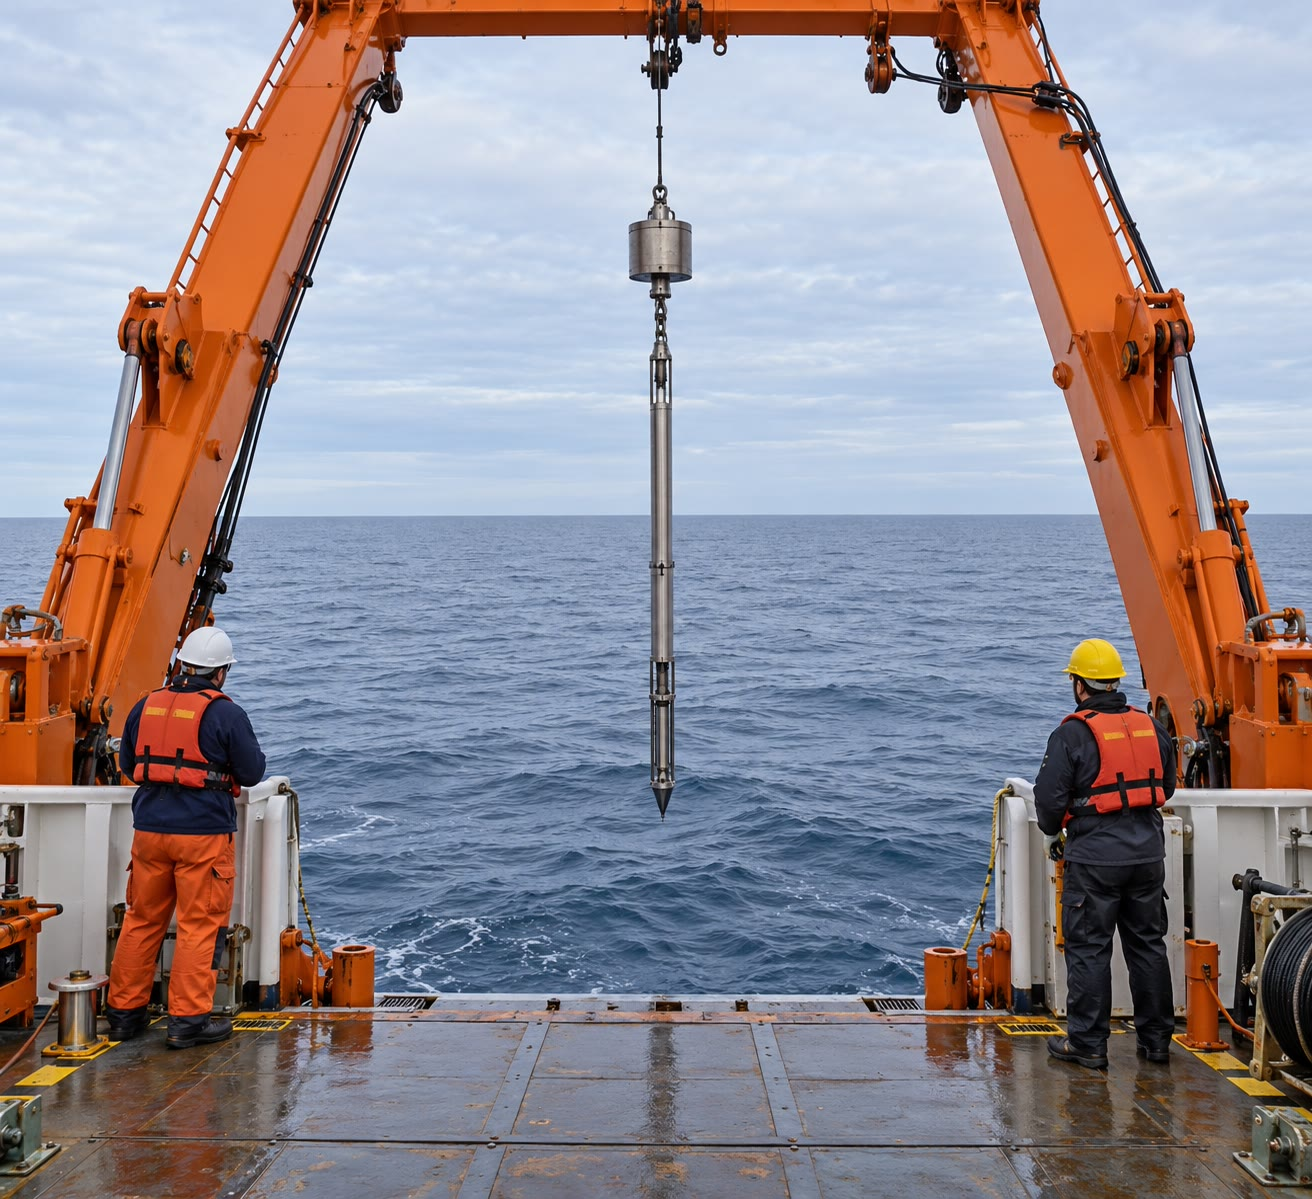
\includegraphics[width=\linewidth]{images/book3/ai/b1-heatflow-probe.jpg}

{\scriptsize शोध-जहाज़ की पिछली क्रेन से लटकता एक ऊष्मा-प्रवाह-प्रोब (AI से बनाया गया चित्र)।}
\end{minipage}
\end{inthefield}

\section{स्थिर चालक जियोथर्म}

\begin{definition}[जियोथर्म]\label{def:b1:heat-budget:geotherm}
सतह के किसी बिंदु के नीचे \emph{जियोथर्म}\index{जियोथर्म} गहराई के फलन के रूप में वहाँ का तापमान, $T(z)$, है। वह एक स्थिर चालक जियोथर्म है जब वह समय के साथ नहीं बदलता और ऊष्मा उसके साथ केवल चालन से ले जाई जाती है।
\end{definition}

\omterm{def:b1:layered-earth:lithosphere}{स्थलमंडल} के भीतर, सक्रिय ज्वालामुखियों और जल-परिसंचरण से दूर, ऊष्मा चालन से ले जाई जाती है, और लाखों वर्षों के पैमाने पर \omterm{def:b1:heat-budget:geotherm}{जियोथर्म} स्थिर है। तब उसका आकार ऊर्जा-संतुलन से निकलता है।

\begin{theorem}[स्थिर चालन और ऊष्मा-उत्पादन]\label{thm:b1:heat-budget:balance}
एक स्थिर चालक \omterm{def:b1:heat-budget:geotherm}{जियोथर्म} के साथ, एकसमान चालकता $k$ और ऊष्मा-उत्पादन $A(z)$ वाले माध्यम में, और ऊष्मा का कोई क्षैतिज प्रवाह न हो,
\[
  \frac{\mathrm dq}{\mathrm dz} = -A(z), \qquad\text{अर्थात्}\qquad
  k\,\frac{\mathrm d^2T}{\mathrm dz^2} = -A(z).
\]
\end{theorem}

\begin{proof}
एक क्षैतिज स्लैब लीजिए जिसका क्षेत्रफल $S$ है और जो गहराइयों $z$ और $z +
\mathrm dz$ के बीच है। ऊष्मा उसके तल से दर $q(z + \mathrm dz)\,S$ पर प्रवेश करती है, ऊपर से दर $q(z)\,S$ पर निकलती है, और भीतर दर $A(z)\,S\,\mathrm dz$ पर उत्पन्न होती है। स्थिर अवस्था में कोई ऊष्मा संचित नहीं होती, अतः $q(z)\,S = q(z + \mathrm dz)\,S + A(z)\,S\,\mathrm dz$, जिससे $\mathrm dq/\mathrm dz = -A$ मिलता है। फ़ूरिये के नियम से $q = k\,\mathrm dT/\mathrm dz$, और $k$ एकसमान होने से, $k\,T'' = -A$।
\end{proof}

सतह से नीचे पढ़ें तो \omterm{def:b1:heat-budget:heat-flow}{ऊष्मा-प्रवाह} हर स्तर के ऊपर उत्पन्न ऊष्मा के कारण गहराई के साथ घटता है: सतह को पार करने वाली ऊष्मा नीचे से आने वाली ऊष्मा और रास्ते में उत्पन्न सारी ऊष्मा है। $A$ के दो वितरण बंद रूप देते हैं।

\begin{proposition}[एक एकसमान रेडियोजनिक परत]\label{prop:b1:heat-budget:uniform}
माना ऊष्मा-उत्पादन $A$ है सतह से गहराई $h$ तक, और उससे नीचे शून्य, सतह $T_0$ तापमान पर हो, और सतही \omterm{def:b1:heat-budget:heat-flow}{ऊष्मा-प्रवाह} $q_0$ हो। तब $0 \le z \le h$ के लिए
\[
  q(z) = q_0 - A z, \qquad T(z) = T_0 + \frac{q_0 z}{k} - \frac{A z^2}{2k},
\]
और $h$ के नीचे \omterm{def:b1:heat-budget:heat-flow}{ऊष्मा-प्रवाह} एकसमान है, $q_m = q_0 - A h$, और \omterm{def:b1:heat-budget:geotherm}{जियोथर्म} ढलान $q_m/k$ की एक सीधी रेखा है।
\end{proposition}

\begin{proof}
$\mathrm dq/\mathrm dz = -A$ का $0$ से समाकलन करें, जहाँ $q(0) = q_0$: $q = q_0 -
Az$। तब $\mathrm dT/\mathrm dz = (q_0 - Az)/k$; $T(0) = T_0$ से समाकलित करने पर परवलय मिलता है। $h$ के नीचे $\mathrm dq/\mathrm dz = 0$ और $q$ अपना $h$ पर का मान रखता है।
\end{proof}

\begin{theorem}[घातांकी ऊष्मा-उत्पादन और रैखिक ऊष्मा-प्रवाह संबंध]
\label{thm:b1:heat-budget:exponential}
माना ऊष्मा-उत्पादन गहराई के साथ $A(z) = A_0 e^{-z/D}$ के अनुसार घटता है, \omterm{def:b1:heat-budget:heat-flow}{ऊष्मा-प्रवाह} बहुत गहराई पर $q_m$ की ओर जाता है, और सतह $T_0$ पर हो। तब
\[
  q(z) = q_m + A_0 D\,e^{-z/D}, \qquad
  T(z) = T_0 + \frac{q_m z}{k} + \frac{A_0 D^2}{k}\bigl(1 - e^{-z/D}\bigr),
\]
और सतही \omterm{def:b1:heat-budget:heat-flow}{ऊष्मा-प्रवाह} है
\[
  q_0 = q_m + A_0 D .
\]
\end{theorem}

\begin{proof}
\cref{thm:b1:heat-budget:balance} से, $\mathrm dq/\mathrm dz =
-A_0e^{-z/D}$, अतः $q(z) = A_0 D e^{-z/D} + C$; जब $z \to \infty$, $q \to C$,
अतः $C = q_m$। $z = 0$ पर, $q_0 = q_m + A_0 D$। तब $\mathrm dT/\mathrm dz =
q/k = q_m/k + (A_0D/k)\,e^{-z/D}$, और $0$ से $T(0) = T_0$ के साथ समाकलित करने पर,
$T = T_0 + q_m z/k + (A_0 D^2/k)(1 - e^{-z/D})$।
\end{proof}

अंतिम पंक्ति सतह पर परखा जा सकने वाला एक पूर्वानुमान है। एक क्षेत्र के ग्रेनाइट प्लूटॉन एक ही गहरा \omterm{def:b1:heat-budget:heat-flow}{ऊष्मा-प्रवाह} $q_m$ साझा करते हैं, और यदि वे केवल इस बात में भिन्न हैं कि यूरेनियम, थोरियम और पोटैशियम में वे कितने समृद्ध हैं, तो एक ही गहराई-पैमाना $D$; तब हर प्लूटॉन के ऊपर मापा गया \omterm{def:b1:heat-budget:heat-flow}{ऊष्मा-प्रवाह} उसकी चट्टानों पर मापे गए ऊष्मा-उत्पादन का एक रैखिक फलन होना चाहिए, ढलान $D$ के साथ, जो एक लंबाई है, और अंतःखंड $q_m$ के साथ, न्यूनित \omterm{def:b1:heat-budget:heat-flow}{ऊष्मा-प्रवाह}, जो रेडियोजनिक परत के नीचे से आता है। फ़्रांसिस बर्च ने ऐसी रेखा पहली बार देखी, जो 1968 में रिपोर्ट की गई, और उसी वर्ष तीन प्रांत उनकी रेखाओं से परिभाषित किए गए:
\begin{center}
\small
% ledger: roy:provinces, roy:linear-relation
\begin{tabular}{lcc}
\hline
प्रांत & अंतःखंड $q_m$ (\unit{mW.m^{-2}}) & ढलान $D$ (\unit{km}) \\
\hline
पूर्वी संयुक्त राज्य & 33 & 7.5 \\
बेसिन और रेंज & 59 & 9.4 \\
सिएरा नेवादा & 17 & 10 \\
\hline
\end{tabular}
\end{center}
मापे गए अंतःखंड, जो 0.8, 1.4 और $0.4\times\qty{e-6}{cal.cm^{-2}.s^{-1}}$ के रूप में प्रकाशित हैं, इससे $\qty{1}{\micro cal.cm^{-2}.s^{-1}} = \qty{41.84}{mW.m^{-2}}$ से परिवर्तित किए गए हैं (\cref{exo:b1:heat-budget:4})। ढलानें थोड़ी बदलती हैं, 7 से \qty{10}{km} तक; न्यूनित \omterm{def:b1:heat-budget:heat-flow}{ऊष्मा-प्रवाह} बहुत बदलता है, और उसके मानचित्र दिखाते हैं कि नीचे का \omterm{def:b1:layered-earth:layers}{प्रावार} कहाँ गरम है, जैसे बेसिन और रेंज की खिंची हुई \omterm{def:b1:layered-earth:layers}{भूपर्पटी} के नीचे। \cref{prop:b1:heat-budget:uniform} की एकसमान परत भी एक सीधी रेखा देती है, जिसकी ढलान $h$ है: दोनों मॉडल आँकड़ों से मेल खाते हैं, पर केवल घातांकी मॉडल ही, जब प्लूटॉन भिन्न गहराइयों तक अपरदित होते हैं, उसी ढलान की सीधी रेखा बना रहता है (\cref{exo:b1:heat-budget:10}), और इसीलिए उसे प्राथमिकता दी जाती है।

\begin{omfigure}
\begin{tikzpicture}
\begin{axis}[omdepth, width=0.82\linewidth, height=8.6cm, xmin=0, xmax=1800, ymin=0, ymax=250, axis x line=top, axis y line=left, axis line style={-}, clip=true,
  xlabel={तापमान (\unit{\degreeCelsius})}, ylabel={गहराई (km)},
  tick label style={font=\scriptsize}, label style={font=\small},
  legend style={font=\scriptsize, at={(0.02,0.02)}, anchor=south west, draw=none, fill=white, fill opacity=0.85, text opacity=1},
  legend cell align=left]
\addplot[very thick, black!45] table[x=T, y=depth] {figdata/out/bachelor-1-geotherms-adiabat.dat};
\addlegendentry{प्रावार का रुद्धोष्म}
\addplot[very thick, red!75!black] table[x=T45, y=depth] {figdata/out/bachelor-1-geotherms-continental.dat};
\addlegendentry{$q_0 = \qty{70}{mW.m^{-2}}$}
\addplot[very thick, orange!80!black] table[x=T30, y=depth] {figdata/out/bachelor-1-geotherms-continental.dat};
\addlegendentry{$q_0 = \qty{55}{mW.m^{-2}}$}
\addplot[very thick, green!45!black] table[x=T15, y=depth] {figdata/out/bachelor-1-geotherms-continental.dat};
\addlegendentry{$q_0 = \qty{40}{mW.m^{-2}}$}
\addplot[thick, blue!70!black, densely dashdotted] table[x=T, y=depth] {figdata/out/bachelor-1-geotherms-oceanic.dat};
\addlegendentry{\qty{60}{Myr} पुराना महासागर-तल}
\addplot[thin, dashed, red!75!black, forget plot] table[x=Tc45, y=depth] {figdata/out/bachelor-1-geotherms-continental.dat};
\addplot[thin, dashed, orange!80!black, forget plot] table[x=Tc30, y=depth] {figdata/out/bachelor-1-geotherms-continental.dat};
\addplot[thin, dashed, green!45!black, forget plot] table[x=Tc15, y=depth] {figdata/out/bachelor-1-geotherms-continental.dat};
\draw[densely dotted, black!60] (axis cs:0,35) -- (axis cs:1800,35);
\node[font=\scriptsize, anchor=south east] at (axis cs:1790,35) {मोहो, \qty{35}{km}};
\fill (axis cs:1384.0,70.8) circle (1.6pt);
\fill (axis cs:1403.2,107.8) circle (1.6pt);
\fill (axis cs:1459.7,224.9) circle (1.6pt);
\node[font=\scriptsize, anchor=west] at (axis cs:1420,66) {\qty{71}{km}};
\node[font=\scriptsize, anchor=west] at (axis cs:1440,104) {\qty{108}{km}};
\node[font=\scriptsize, anchor=west] at (axis cs:1495,222) {\qty{225}{km}};
\end{axis}
\end{tikzpicture}

\par\smallskip{\small एक महाद्वीप के स्थिर चालक \omterm{def:b1:heat-budget:geotherm}{जियोथर्म}, जिसमें ऊष्मा-उत्पादन $A_0 = \qty{2.5}{\micro W.m^{-3}}$ है जो $D = \qty{10}{km}$ पर घटता है, $k = \qty{2.5}{W.m^{-1}.K^{-1}}$ के साथ, तीन सतही ऊष्मा-प्रवाहों के लिए (न्यूनित \omterm{def:b1:heat-budget:heat-flow}{ऊष्मा-प्रवाह} 15, 30 और \qty{45}{mW.m^{-2}})। हर एक अपनी चालक वक्र (उसके आगे बिंदुकित) का अनुसरण करता है नीचे \omterm{def:b1:layered-earth:layers}{प्रावार} के रुद्धोष्म तक, जिससे वह बिंदु पर मिलता है: \omterm{def:b1:heat-budget:boundary-layer}{ऊष्मीय स्थलमंडल} का आधार। महासागर-तल का \omterm{def:b1:heat-budget:geotherm}{जियोथर्म} \qty{60}{Myr} तक ठंडे हुए अर्ध-अंतरिक्ष का है। एकसमान चालकता एक सरलीकरण है।}
\label{fig:b1:heat-budget:geotherms}
\end{omfigure}

\begin{method}[प्लूटॉन के नीचे गहराई पर तापमान]\label{met:b1:heat-budget:moho}
\begin{enumerate}
  \item प्लूटॉन के ऊपर सतही \omterm{def:b1:heat-budget:heat-flow}{ऊष्मा-प्रवाह} $q_0$ मापिए (बोरहोल विधि) और उसका ऊष्मा-उत्पादन $A_0$ उसकी U, Th और K मात्राओं से।
  \item प्रांत की रेखा से, या लगभग \qty{10}{km} के $D$ मान से, $q_m = q_0 - A_0 D$ परिकलित कीजिए।
  \item \cref{thm:b1:heat-budget:exponential} लागू कीजिए। कुछ गुना $D$ से नीचे, $e^{-z/D}$ नगण्य है और \omterm{def:b1:heat-budget:geotherm}{जियोथर्म} सीधी रेखा $T_0 + A_0D^2/k + q_m z/k$ है: रेडियोजनिक परत ने हर गहरे तापमान को $A_0D^2/k$ से ऊपर उठा दिया है।
\end{enumerate}
\end{method}

आकृति में \omterm{def:b1:layered-earth:discontinuity}{मोहो} पर तापमान सबसे कम \omterm{def:b1:heat-budget:heat-flow}{ऊष्मा-प्रवाह} के लिए लगभग \qty{320}{\degreeCelsius} से सबसे अधिक के लिए \qty{700}{\degreeCelsius} से ऊपर तक है: सतह पर का \omterm{def:b1:heat-budget:heat-flow}{ऊष्मा-प्रवाह} गहरी \omterm{def:b1:layered-earth:layers}{भूपर्पटी} के तापमान का सीधा पाठ देता है, जो उसकी सामर्थ्य को नियंत्रित करता है (\cref{ch:b1:stress-strain-rheology})।

\section{चालन बनाम संवहन}

चालन धीमा है। यह कितना धीमा है, वह ऊष्मा-समीकरण से निकलता है, जिसे भौतिकी की पुस्तकें फ़ूरिये के नियम और \cref{thm:b1:heat-budget:balance} के संतुलन से संचय जोड़कर व्युत्पन्न करती हैं: एक आयाम में, ऊष्मा-उत्पादन के बिना,
$\partial T/\partial t = \kappa\,\partial^2 T/\partial z^2$.

\begin{proposition}[चालन का समय-पैमाना]\label{prop:b1:heat-budget:timescale}
किसी चालक पिंड की सीमा पर आरोपित एक तापमान-परिवर्तन दूरी $L$ तक फैलता है, एक ऐसे समय में जिसका क्रम है
\[
  \tau = \frac{L^2}{\kappa} .
\]
\end{proposition}

\begin{proof}
माना $z = L z^*$, $t = \tau t^*$, जहाँ $z^*$ और $t^*$ विमाहीन हैं। ऊष्मा-समीकरण इस रूप में बन जाता है $\partial T/\partial t^* = (\kappa\tau/L^2)\,\partial^2
T/\partial z^{*2}$। इसके हल पैमाने $z^* \sim 1$ पर तब बदलते हैं जब $t^* \sim 1$ हो, केवल तभी जब गुणांक एक के क्रम का हो, अर्थात् यदि $\tau \sim L^2/\kappa$ हो।
\end{proof}

चट्टानों में $\kappa \approx \qty{e-6}{m^2.s^{-1}}$ है। दैनिक तापमान-चक्र ज़मीन में कुछ दसियों सेंटीमीटर तक पहुँचता है, वार्षिक चक्र कुछ मीटर तक, और अंतिम हिमयुग से हुआ तापन लगभग एक किलोमीटर तक। \qty{100}{km} मोटे \omterm{def:b1:layered-earth:lithosphere}{स्थलमंडल} के आर-पार $\tau = \qty{e16}{s}$, लगभग \qty{300}{Myr}। \qty{2900}{km} मोटे \omterm{def:b1:layered-earth:layers}{प्रावार} के आर-पार $\tau = \qty{8.4e18}{s}$, या \qty{270}{Gyr}: पृथ्वी की आयु \qty{4.54}{Gyr} से साठ गुना। % ledger: england:kelvin, usgs:age-earth
चालन अकेला गहरे \omterm{def:b1:layered-earth:layers}{प्रावार} की ऊष्मा को सतह के कहीं पास नहीं ला सकता था। \omterm{def:b1:layered-earth:layers}{प्रावार} संवहन करता है, और उसके भीतर ऊष्मा चट्टान की अपनी गति से ले जाई जाती है, प्लेटों की चाल से, सेंटीमीटर प्रति वर्ष। % ledger: usgs:san-andreas

\begin{definition}[प्रावार रुद्धोष्म]\label{def:b1:heat-budget:adiabat}
\emph{प्रावार रुद्धोष्म}\index{प्रावार रुद्धोष्म} संवहन करते \omterm{def:b1:layered-earth:layers}{प्रावार} के अच्छी तरह मिश्रित भीतरी भाग का \omterm{def:b1:heat-budget:geotherm}{जियोथर्म} है: वह तापमान जो \omterm{def:b1:layered-earth:layers}{प्रावार} की चट्टान तब लेती है जब वह इतनी तेज़ी से ऊपर उठती या नीचे धँसती है कि अपने परिवेश से कोई ऊष्मा का आदान-प्रदान न करे, ऊपर उठते समय विस्तार से ठंडी होती हुई और नीचे धँसते समय संपीड़न से गरम होती हुई।
\end{definition}

ऊष्मागतिकी इसकी प्रवणता देती है, $\mathrm dT/\mathrm dz = \alpha g T/c_p$, जहाँ $\alpha$ ऊष्मीय प्रसार-गुणांक है और $c_p$ विशिष्ट ऊष्मा (भौतिकी से, यहाँ स्वीकृत)। यह छोटी है। खनिज-भौतिकी से एक हाल का मूल्यांकन \qty{50}{km} गहराई पर \qty{0.54}{K.km^{-1}} देता है, जो \qty{410}{km} पर \qty{0.36}{K.km^{-1}} तक घटती है, फिर निचले \omterm{def:b1:layered-earth:layers}{प्रावार} में 0.41 से \qty{0.23}{K.km^{-1}} तक, \qty{50}{km} पर \qty{1646}{K} और \qty{2800}{km} पर \qty{2587}{K} के साथ।
% ledger: katsura:adiabat
सतह तक बाहर की ओर बढ़ाने पर रुद्धोष्म \omterm{def:b1:layered-earth:layers}{प्रावार} का विभव-तापमान देता है, \qty{1619}{K} या लगभग \qty{1350}{\degreeCelsius}: वह तापमान जो \omterm{def:b1:layered-earth:layers}{प्रावार} का होता यदि उसे बिना ऊष्मा का आदान-प्रदान किए सतह तक लाया जाता। विभव-तापमान की धारणा वायुमंडल और महासागर के लिए \cref{ch:b1:fluid-envelopes-structure} में परिभाषित होती है। एक तापमान जो प्रति किलोमीटर केवल \qty{0.5}{K} बढ़ता है, जबकि सतह के पास का चालक \omterm{def:b1:heat-budget:geotherm}{जियोथर्म} \qty{25}{K} चढ़ता है, संवहन का चिह्न है।

\begin{history}[जॉन पेरी और शीतल होती पृथ्वी]
1862--1863 में विलियम थॉमसन, जो बाद में लॉर्ड केल्विन बने, ने ठंडे होने से पृथ्वी की आयु परिकलित की। उन्होंने इसे एक ठोस माना जो लगभग \qty{3900}{\degreeCelsius} के एकसमान तापमान से चालन द्वारा ठंडा हुआ; उस समय के मापों से उन्होंने जो औसत प्रवणता चुनी, लगभग \qty{36}{K.km^{-1}}, और \qty{1.2e-6}{m^2.s^{-1}} के विसरणशीलता-मान के साथ, आज की प्रवणता तक पहुँचने का समय लगभग \qty{96}{Myr} था, 24 और \qty{400}{Myr} की सीमाओं के बीच (\cref{exo:b1:heat-budget:9})। भूवैज्ञानिकों को यह बहुत कम लगा। 1895 में, रेडियोधर्मिता की खोज से एक वर्ष पहले, उनके पूर्व सहायक जॉन पेरी ने इसके बजाय एक धारणा की ओर इशारा किया: यदि भीतरी भाग आंशिक रूप से द्रव और संवहनी होता, तो वह ऊष्मा ऐसे ले जाता मानो उसकी चालकता अपार हो, और पूरा भीतरी भाग, न कि एक पतला बाहरी कवच, सतह के \omterm{def:b1:heat-budget:heat-flow}{ऊष्मा-प्रवाह} को पोषित करता। उनका तर्क उपेक्षित और भुला दिया गया; बहुत बाद में स्थापित प्रावार-संवहन ने उन्हें सही सिद्ध किया: गहरा \omterm{def:b1:layered-earth:layers}{प्रावार} संवहन द्वारा ठंडा होता है, और यही बजट का \omterm{def:b1:heat-budget:secular-cooling}{दीर्घकालिक शीतलन} है। % ledger: england:kelvin, england:perry
\end{history}

\begin{proposition}[पेरी की अच्छी तरह मिश्रित पृथ्वी]\label{prop:b1:heat-budget:perry}
त्रिज्या $R$ का एक गोला लीजिए जिसका भीतरी भाग एकसमान तापमान $T_i(t)$ पर अच्छी तरह मिश्रित हो, प्रति इकाई आयतन ऊष्मा-धारिता $\rho c$ के साथ, $L \ll R$ मोटाई और चालकता $k$ वाले एक चालक ढक्कन के नीचे, जिसकी सतह $\qty{0}{\degreeCelsius}$ पर है, और मान लीजिए कोई ऊष्मा-उत्पादन नहीं है। तब
\[
  T_i(t) = T_i(0)\,e^{-t/\tau_P}, \qquad \tau_P = \frac{RL}{3\kappa},
\]
और सतही \omterm{def:b1:heat-budget:heat-flow}{ऊष्मा-प्रवाह} $kT_i/L$ उसी समय-स्थिरांक के साथ क्षय होता है।
\end{proposition}

\begin{proof}
ढक्कन पतला होने से वह साम्य में है और \omterm{def:b1:heat-budget:heat-flow}{ऊष्मा-प्रवाह} $q = kT_i/L$ ढोता है। भीतरी भाग क्षेत्रफल $4\pi R^2$ से होकर अपनी ऊष्मा खोता है: $\tfrac43\pi R^3\rho c\,\mathrm dT_i/\mathrm dt = -4\pi R^2 kT_i/L$, अर्थात् $\mathrm dT_i/\mathrm dt = -3\kappa T_i/(RL)$ जहाँ $\kappa = k/(\rho c)$, जिसका हल $\tau_P = RL/(3\kappa)$ वाला घातांक है।
\end{proof}

$R = \qty{6400}{km}$, $L = \qty{100}{km}$ और $\kappa =
\qty{e-6}{m^2.s^{-1}}$ के लिए, $\tau_P = \qty{6.8}{Gyr}$: संवहन करती पृथ्वी अरबों वर्षों तक ऊँचा \omterm{def:b1:heat-budget:heat-flow}{ऊष्मा-प्रवाह} बनाए रखती है, जहाँ केल्विन की चालक पृथ्वी उसे दसियों लाख वर्षों में खो देती थी (\cref{exo:b1:heat-budget:11})।

\section{स्थलमंडल एक ऊष्मीय सीमा-परत के रूप में}\label{sec:b1:heat-budget:boundary-layer}

\begin{definition}[ऊष्मीय सीमा-परत, ऊष्मीय स्थलमंडल]\label{def:b1:heat-budget:boundary-layer}
एक संवहनी द्रव में, एक \emph{ऊष्मीय सीमा-परत}\index{ऊष्मीय सीमा-परत} एक सीमा के साथ की ऐसी परत है जिसके आरपार ऊष्मा चालन से गुज़रती है और तापमान सीमा के तापमान से अच्छी तरह मिश्रित भीतरी भाग के तापमान तक बदलता है। \emph{ऊष्मीय स्थलमंडल}\index{ऊष्मीय स्थलमंडल} \omterm{def:b1:layered-earth:layers}{प्रावार} की ऊपरी ऊष्मीय सीमा-परत है: सतह से लेकर उस गहराई तक का पृथ्वी का बाहरी कवच जहाँ चालक \omterm{def:b1:heat-budget:geotherm}{जियोथर्म} \omterm{def:b1:heat-budget:adiabat}{प्रावार रुद्धोष्म} से मिलता है।
\end{definition}

प्लेटें \omterm{def:b1:layered-earth:layers}{प्रावार} के संवहन का ठंडा ऊपरी भाग हैं, उसकी ऊपरी सीमा-परत। उनका आधार, जहाँ तीखा चालक \omterm{def:b1:heat-budget:geotherm}{जियोथर्म} मंद रुद्धोष्म में मुड़ता है, \qtyrange{70}{230}{km} पर है, 70 से \qty{40}{mW.m^{-2}} तक महाद्वीपीय ऊष्मा-प्रवाहों के जियोथर्म-चित्र में, भूकंप-विज्ञान से मापी गई परास में (\cref{ch:b1:layered-earth}): अपनी सामर्थ्य से परिभाषित \omterm{def:b1:layered-earth:lithosphere}{स्थलमंडल} और अपने तापमान से परिभाषित \omterm{def:b1:layered-earth:lithosphere}{स्थलमंडल} लगभग एक ही कवच हैं, क्योंकि सामर्थ्य तापमान पर निर्भर करती है। \omterm{def:b1:layered-earth:layers}{प्रावार} के तल पर, D$''$ परत निचली सीमा-परत है, जिसे नीचे से कोर गरम करता है।

महासागरों के नीचे \omterm{def:b1:heat-budget:boundary-layer}{ऊष्मीय सीमा-परत} कटक पर जन्म लेती है, जहाँ गरम \omterm{def:b1:layered-earth:layers}{प्रावार} सतह तक उठता है, और जैसे-जैसे प्लेट दूर खिसकती और ठंडी होती है, वह मोटी होती है। एकसमान तापमान से एक अर्ध-अंतरिक्ष का शीतलन, जिसे फ़ूरिये ने हल किया और केल्विन ने पूरी पृथ्वी के लिए प्रयोग किया, इसे अच्छी तरह वर्णित करता है (\cref{ch:b1:rifts-ridges-margins} और तीसरे वर्ष का खंड इसे व्युत्पन्न करता है): समतापीय रेखाएँ तल की आयु के वर्गमूल के अनुपात में गहरी होती हैं (नीचे का चित्र), और \omterm{def:b1:heat-budget:heat-flow}{ऊष्मा-प्रवाह} घटता है:
\[
  q(t) = \frac{C}{\sqrt t}, \qquad C \approx \qty{490}{mW.m^{-2}.Myr^{1/2}},
\]
वैश्विक बजट में प्रयुक्त मान। % ledger: dd10:young-ocean
\qty{100}{Myr} पर अर्ध-अंतरिक्ष लगभग \qty{130}{km} तक ठंडा हो गया है (\cref{exo:b1:heat-budget:12})। वास्तविक प्लेट पहले मोटी होना बंद कर देती है: प्रशांत पर से गुज़रती भूकंपीय तरंगें एक ऐसी ठंडी होती प्लेट से सबसे अच्छी तरह मेल खाती हैं जो \qtyrange{85}{95}{km} की मोटाई की ओर जाती है, पुराने समुद्र-तल का वह चपटापन जो \cref{ch:b1:rifts-ridges-margins} में फिर मिलता है।
% ledger: fischer:lithosphere

ऊष्मा-बजट, प्लेटों का \omterm{def:b1:heat-budget:heat-flow}{ऊष्मा-प्रवाह} और ऊष्मीय संरचना अगले अध्यायों में एक साथ आते हैं: ठंडी होती प्लेट धँसती है (\cref{ch:b1:rifts-ridges-margins}), और उप-संवहन क्षेत्रों पर धँसता ठंडा \omterm{def:b1:layered-earth:lithosphere}{स्थलमंडल} उस संवहन का अधोगामी प्रवाह है जिसका वह हिस्सा है।

\begin{omfigure}
\begin{tikzpicture}
\begin{axis}[width=0.86\linewidth, height=5.6cm, xmin=0, xmax=100, ymin=0, ymax=170,
  y dir=reverse, axis x line=top, axis y line=left, axis line style={-}, clip=false,
  xlabel={महासागर-तल की आयु (\unit{Myr}), कटक से दूरी के साथ बढ़ती},
  ylabel={गहराई (km)}, tick label style={font=\scriptsize}, label style={font=\small}]
\addplot[fill=blue!12, draw=none] table[x=age, y=z1200] {figdata/out/bachelor-1-geotherms-isotherms.dat} \closedcycle;
\addplot[thick, blue!30!black] table[x=age, y=z400] {figdata/out/bachelor-1-geotherms-isotherms.dat};
\addplot[thick, blue!50!red] table[x=age, y=z800] {figdata/out/bachelor-1-geotherms-isotherms.dat};
\addplot[very thick, red!75!black] table[x=age, y=z1200] {figdata/out/bachelor-1-geotherms-isotherms.dat};
\node[font=\scriptsize, anchor=south, fill=blue!12, inner sep=1pt] at (axis cs:80,24) {\qty{400}{\degreeCelsius}};
\node[font=\scriptsize, anchor=south, fill=blue!12, inner sep=1pt] at (axis cs:80,55) {\qty{800}{\degreeCelsius}};
\node[font=\scriptsize, anchor=south, fill=blue!12, inner sep=1pt] at (axis cs:80,108) {\qty{1200}{\degreeCelsius}};
\node[font=\small] at (axis cs:60,72) {ऊष्मीय स्थलमंडल};
\node[font=\small] at (axis cs:55,150) {संवहनी प्रावार, लगभग \qty{1350}{\degreeCelsius}};
\draw[->, thick, red!60!black] (axis cs:3,165) -- (axis cs:3,125);
\node[font=\scriptsize, anchor=west, red!60!black] at (axis cs:4,140) {कटक के नीचे ऊपर उठता};
\draw[->, thick, black!60] (axis cs:30,5) -- (axis cs:70,5);
\node[font=\scriptsize, anchor=west] at (axis cs:70,5) {प्लेट की गति};
\end{axis}
\end{tikzpicture}

\par\smallskip{\small महासागरीय प्लेट के ठंडे होते समय समतापीय रेखाएँ: आरंभ में \qty{1350}{\degreeCelsius} पर एक अर्ध-अंतरिक्ष, अपनी सतह से ठंडा होता हुआ, जिसमें $\kappa = \qty{e-6}{m^2.s^{-1}}$ है। हर समतापीय रेखा आयु के वर्गमूल के अनुपात में गहरी होती है; \qty{1200}{\degreeCelsius} की समतापीय रेखा के ऊपर की छायांकित परत \omterm{def:b1:heat-budget:boundary-layer}{ऊष्मीय स्थलमंडल} है। तीर योजनाबद्ध हैं।}
\label{fig:b1:heat-budget:isotherms}
\end{omfigure}

\section{अभ्यास}

\begin{exercise}[$\star$]\label{exo:b1:heat-budget:1}
\qty{2.5}{W.m^{-1}.K^{-1}} चालकता वाले ग्रेनाइट में एक बोरहोल \qty{22}{K.km^{-1}} की स्थिर प्रवणता दिखाता है। \omterm{def:b1:heat-budget:heat-flow}{ऊष्मा-प्रवाह}, और वहाँ सतह के एक वर्ग किलोमीटर को पार करने वाली शक्ति परिकलित कीजिए।
% ledger: delaney:conductivity
\end{exercise}

\begin{exercise}[$\star$]\label{exo:b1:heat-budget:2}
महाद्वीपों (\qty{2.073e14}{m^2}, \qty{70.9}{mW.m^{-2}}) और महासागरों (\qty{3.028e14}{m^2}, \qty{105.4}{mW.m^{-2}}) के क्षेत्रफलों और औसत ऊष्मा-प्रवाहों से, हर एक की ऊष्मा-हानि, और पृथ्वी की सतह (\qty{5.101e14}{m^2}) पर कुल तथा औसत \omterm{def:b1:heat-budget:heat-flow}{ऊष्मा-प्रवाह} परिकलित कीजिए। सूर्य से प्राप्त \qty{173000}{TW} का वह कितना भाग है?
% ledger: dd10:split, nasa:solar-mean
\end{exercise}

\begin{exercise}[$\star$]\label{exo:b1:heat-budget:3}
चार समस्थानिकों की सारणी से, प्राकृतिक यूरेनियम के प्रति किलोग्राम (परमाणुओं का \qty{99.274}{\percent} \ce{^{238}U} और \qty{0.720}{\percent} \ce{^{235}U}; उनके द्रव्यमान लगभग \qty{1}{\percent} भिन्न हैं, अतः इन्हें द्रव्यमान-अंश मानिए) और प्राकृतिक पोटैशियम के प्रति किलोग्राम की ऊष्मा परिकलित कीजिए, जिसका \ce{^{40}K} परमाणुओं का \qty{0.0117}{\percent} बनाता है (एक \ce{^{40}K} परमाणु का द्रव्यमान पोटैशियम परमाणु के औसत द्रव्यमान का $39.96/39.10$ गुना मानिए)।
% ledger: dye:isotope-heat, iaea:isotopes
\end{exercise}

\begin{exercise}[$\star$]\label{exo:b1:heat-budget:4}
तीन प्रांतों के अंतःखंड, 0.8, 1.4 और $0.4\times\qty{e-6}{cal.cm^{-2}.s^{-1}}$, को \unit{mW.m^{-2}} में बदलिए ($\qty{1}{cal} = \qty{4.184}{J}$)। हर प्रांत में \qty{3.0}{\micro W.m^{-3}} ऊष्मा-उत्पादन वाले एक ग्रेनाइट के ऊपर सतही \omterm{def:b1:heat-budget:heat-flow}{ऊष्मा-प्रवाह} का पूर्वानुमान लगाइए।
% ledger: roy:provinces
\end{exercise}

\begin{exercise}[$\star\star$]\label{exo:b1:heat-budget:5}
एक \omterm{def:b1:layered-earth:layers}{भूपर्पटी} में ऊपरी \qty{10}{km} में एकसमान ऊष्मा-उत्पादन \qty{2.0}{\micro W.m^{-3}} है और नीचे कोई नहीं, चालकता \qty{2.5}{W.m^{-1}.K^{-1}}, सतही \omterm{def:b1:heat-budget:heat-flow}{ऊष्मा-प्रवाह} \qty{60}{mW.m^{-2}} और सतह-तापमान \qty{10}{\degreeCelsius}। \qty{10}{km} पर तापमान, रेडियोजनिक परत के नीचे \omterm{def:b1:heat-budget:heat-flow}{ऊष्मा-प्रवाह}, और \qty{35}{km} नीचे \omterm{def:b1:layered-earth:discontinuity}{मोहो} पर तापमान परिकलित कीजिए।
\end{exercise}

\begin{exercise}[$\star\star$]\label{exo:b1:heat-budget:6}
एक बोरहोल \qty{300}{m} शेल ($k = \qty{1.5}{W.m^{-1}.K^{-1}}$) और फिर ग्रेनाइट ($k = \qty{3.0}{W.m^{-1}.K^{-1}}$) पार करता है। \omterm{def:b1:comparative-planetology:equilibrium-temperature}{साम्य तापमान} सतह पर \qty{12.0}{\degreeCelsius}, \qty{300}{m} पर \qty{24.0}{\degreeCelsius} और \qty{800}{m} पर \qty{34.0}{\degreeCelsius} हैं। हर चट्टान में प्रवणता और \omterm{def:b1:heat-budget:heat-flow}{ऊष्मा-प्रवाह}, \qty{300}{m} और \qty{800}{m} पर ऊष्मीय प्रतिरोध, और बुलार्ड आलेख की ढलान परिकलित कीजिए। क्या \omterm{def:b1:heat-budget:heat-flow}{ऊष्मा-प्रवाह} स्थिर है?
\end{exercise}

\begin{exercise}[$\star\star$]\label{exo:b1:heat-budget:7}
$\kappa = \qty{e-6}{m^2.s^{-1}}$ के साथ, $L = \qty{1}{m}$, \qty{10}{m}, \qty{100}{km} और \qty{2900}{km} के लिए चालक समय-पैमाना परिकलित कीजिए, हर एक उपयुक्त इकाई में। \qty{10}{m} नीचे ज़मीन में कौन-से सतही तापमान-चक्र अब भी महसूस होते हैं? अंतिम समय की पृथ्वी की आयु से तुलना कीजिए।
% ledger: england:kelvin, usgs:age-earth
\end{exercise}

\begin{exercise}[$\star\star$]\label{exo:b1:heat-budget:8}
\omterm{def:b1:heat-budget:adiabat}{प्रावार रुद्धोष्म} \qty{50}{km} गहराई पर \qty{1646}{K} पर है, वहाँ \qty{0.54}{K.km^{-1}} की प्रवणता के साथ, जो \qty{410}{km} पर \qty{0.36}{K.km^{-1}} तक घटती है। (क) इसे \qty{50}{km} की प्रवणता के साथ सतह तक बढ़ाइए, और विभव-तापमान केल्विन और डिग्री सेल्सियस में दीजिए। (ख) दो प्रवणताओं के माध्य से \qty{410}{km} पर तापमान का अनुमान लगाइए, और उसकी तुलना असांतत्य के ठीक ऊपर प्रकाशित \qty{1799}{K} से कीजिए।
% ledger: katsura:adiabat
\end{exercise}

\begin{exercise}[$\star\star$]\label{exo:b1:heat-budget:9}
एकसमान तापमान $T_0$ से ठंडा हुआ एक अर्ध-अंतरिक्ष, जिसकी सतह $\qty{0}{\degreeCelsius}$ पर रखी गई है, समय $t$ के बाद सतही प्रवणता $G =
T_0/\sqrt{\pi\kappa t}$ रखता है (स्वीकृत)। (क) $t$ को $G$ के पदों में व्यक्त कीजिए। (ख) केल्विन के मानों के साथ, $T_0 = \qty{3900}{\degreeCelsius}$, $\kappa =
\qty{1.2e-6}{m^2.s^{-1}}$ और $G = 1/50$ डिग्री फ़ारेनहाइट प्रति फ़ुट: $G$ को \unit{K.km^{-1}} में और आयु परिकलित कीजिए। (ग) इसे $T_0 =
\qty{1300}{\degreeCelsius}$, $\kappa = \qty{e-6}{m^2.s^{-1}}$ और $G =
\qty{36}{K.km^{-1}}$ के साथ फिर कीजिए।
% ledger: england:kelvin
\end{exercise}

\begin{exercise}[$\star\star\star$]\label{exo:b1:heat-budget:10}
एक प्रांत का क्षरण होता है: हर प्लूटॉन के ऊपर से मोटाई $e$ हटती है, जबकि गहरा \omterm{def:b1:heat-budget:heat-flow}{ऊष्मा-प्रवाह} $q_m$ अपरिवर्तित रहता है। (क) घातांकी मॉडल में दिखाइए कि नए सतही ऊष्मा-उत्पादन और \omterm{def:b1:heat-budget:heat-flow}{ऊष्मा-प्रवाह}, $A_0'$ और $q_0'$, अब भी $q_0' = q_m + A_0'D$ को संतुष्ट करते हैं। (ख) मोटाई $h$ की एकसमान-परत मॉडल में दिखाइए कि $e$ से क्षरित प्लूटॉन ढलान $h - e$ की रेखा पर स्थित है। (ग) एक प्रांत के प्लूटॉन भिन्न मात्राओं से क्षरित हुए। कौन-सा मॉडल भविष्यवाणी करता है कि वे अब भी एक ही रेखा पर गिरते हैं?
\end{exercise}

\begin{exercise}[$\star\star\star$]\label{exo:b1:heat-budget:11}
पेरी के मॉडल (\cref{prop:b1:heat-budget:perry}) में $R = \qty{6400}{km}$, $\kappa = \qty{e-6}{m^2.s^{-1}}$, $k = \qty{3}{W.m^{-1}.K^{-1}}$ और \qty{1300}{\degreeCelsius} का आरंभिक भीतरी तापमान लीजिए। (क) \qty{50}{km} और \qty{100}{km} के ढक्कनों के लिए $\tau_P$ परिकलित कीजिए। (ख) \qty{50}{km} वाले ढक्कन के लिए, आरंभ में और \qty{2}{Gyr} के बाद सतही \omterm{def:b1:heat-budget:heat-flow}{ऊष्मा-प्रवाह} परिकलित कीजिए। (ग) वही $k$ और $T_0$ रखने वाले केल्विन के चालक अर्ध-अंतरिक्ष का सतही \omterm{def:b1:heat-budget:heat-flow}{ऊष्मा-प्रवाह} $kT_0/\sqrt{\pi\kappa t}$ है: उसे \qty{2}{Gyr} के बाद परिकलित कीजिए, और तुलना कीजिए।
% ledger: england:kelvin, england:perry
\end{exercise}

\begin{exercise}[$\star\star\star$]\label{exo:b1:heat-budget:12}
शीतल होते अर्ध-अंतरिक्ष का सतही \omterm{def:b1:heat-budget:heat-flow}{ऊष्मा-प्रवाह} $q = k\,\Delta T/\sqrt{\pi\kappa t}$ है (\cref{exo:b1:heat-budget:9})। (क) $k = \qty{3}{W.m^{-1}.K^{-1}}$, $\kappa =
\qty{e-6}{m^2.s^{-1}}$ और $\Delta T = \qty{1336}{K}$ के साथ (विभव-तापमान से लगभग \qty{10}{\degreeCelsius} पर समुद्र-तल तक), $C$, जो $q = C/\sqrt t$ में स्थिरांक है, $t$ को करोड़ों वर्षों में मानकर, परिकलित कीजिए, और उसकी तुलना आँकड़ों पर फ़िट \qty{490}{mW.m^{-2}.Myr^{1/2}} से कीजिए। (ख) $C = 490$ लेकर \qty{1}{Myr}, \qty{10}{Myr} और \qty{100}{Myr} पर \omterm{def:b1:heat-budget:heat-flow}{ऊष्मा-प्रवाह} दीजिए। (ग) शीतलन समतापीय रेखाओं के चित्र की \qty{1200}{\degreeCelsius} समतापीय रेखा वहाँ स्थित है जहाँ $z = 2\times1.163\sqrt{\kappa t}$; \qty{100}{Myr} पर उसकी गहराई परिकलित कीजिए।
% ledger: dd10:young-ocean, katsura:adiabat, fischer:lithosphere
\end{exercise}

\section{समस्या: प्लूटॉनों के नीचे गरम चट्टानें}

\begin{problem}[{सप्ताहांत समस्या --- पाँच ग्रेनाइट प्लूटॉनों का ऊष्मा-प्रवाह और ऊष्मा-उत्पादन, रैखिक संबंध, और गहरी भूपर्पटी का तापमान}]
\label{pb:b1:heat-budget:1}
% values: calc/ch10.py (invented province; element heats from the chapter's table)
% ledger: dye:isotope-heat, iaea:isotopes, dd10:split, roy:provinces
एक प्रांत के पाँच ग्रेनाइट प्लूटॉनों में ड्रिलिंग की गई है। हर बोरहोल में साम्य-तापमान \qty{100}{m} और \qty{500}{m} पर दर्ज किया गया, और ग्रेनाइट की चालकता कोर-नमूनों पर मापी गई; उसकी यूरेनियम, थोरियम और पोटैशियम मात्राएँ सतही नमूनों पर विश्लेषित की गईं। पाँचों ग्रेनाइटों का घनत्व \qty{2650}{kg.m^{-3}} है।
\begin{center}
\small
\begin{tabular}{cccccc}
\hline
प्लूटॉन & $T$ पर \qty{100}{m} (\unit{\degreeCelsius}) & $T$ पर \qty{500}{m} (\unit{\degreeCelsius}) & $k$ (\unit{W.m^{-1}.K^{-1}}) & U, Th (ppm) & K (\unit{\percent}) \\
\hline
A & 13.1 & 19.2 & 2.9 & 2.0, 8 & 3.0 \\
B & 12.4 & 20.2 & 2.6 & 3.5, 14 & 3.5 \\
C & 13.6 & 21.4 & 3.1 & 5.0, 18 & 4.0 \\
D & 12.9 & 23.1 & 2.7 & 7.0, 25 & 4.2 \\
E & 14.2 & 25.5 & 3.0 & 10.0, 35 & 4.5 \\
\hline
\end{tabular}
\end{center}
तत्व-ऊष्माएँ $\qty{9.85e-5}{W.kg^{-1}}$ (U), $\qty{2.63e-5}{W.kg^{-1}}$ (Th) और $\qty{3.40e-9}{W.kg^{-1}}$ (K) लीजिए। प्लूटॉनों के नीचे, पूरी \omterm{def:b1:layered-earth:layers}{भूपर्पटी} के लिए $k = \qty{2.5}{W.m^{-1}.K^{-1}}$ और \qty{10}{\degreeCelsius} सतह-तापमान लीजिए।

\medskip
\noindent\textbf{भाग I --- ऊष्मा-प्रवाह।}
\begin{enumerate}
  \item हर बोरहोल में तापमान-प्रवणता परिकलित कीजिए।
  \item तापमानों को ड्रिलिंग के सप्ताहों या महीनों बाद ही क्यों दर्ज करना चाहिए, और सबसे ऊपर की \qty{100}{m} क्यों छोड़ी जाती है?
  \item हर प्लूटॉन पर \omterm{def:b1:heat-budget:heat-flow}{ऊष्मा-प्रवाह} परिकलित कीजिए।
  \item उन्हें औसत महाद्वीपीय \omterm{def:b1:heat-budget:heat-flow}{ऊष्मा-प्रवाह}, \qty{70.9}{mW.m^{-2}} से तुलना कीजिए।
  \item B और C की प्रवणताएँ बराबर हैं। उनके \omterm{def:b1:heat-budget:heat-flow}{ऊष्मा-प्रवाह} क्यों बराबर नहीं हैं?
  \item प्लूटॉन पहाड़ियों के नीचे हैं। क्या उच्चावच किसी शिखर के नीचे मापी गई प्रवणता को बढ़ाता या घटाता? (समतापीय रेखाओं के आकार पर सोचिए।)
\end{enumerate}

\noindent\textbf{भाग II --- ऊष्मा-उत्पादन और रेखा।}
\begin{enumerate}[resume]
  \item हर प्लूटॉन में यूरेनियम के कारण ऊष्मा-उत्पादन परिकलित कीजिए।
  \item थोरियम के लिए वही।
  \item पोटैशियम के लिए वही।
  \item इन्हें जोड़कर हर प्लूटॉन के लिए $A_0$ प्राप्त कीजिए। कौन-सा तत्व सबसे कम योगदान देता है?
  \item $q_0$ को $A_0$ के विरुद्ध खींचिए। क्या बिंदु किसी सीधी रेखा के निकट पड़ते हैं?
  \item $A_0$ और $q_0$ के माध्य, और योग $\sum (A_0 - \bar A_0)^2$ और $\sum (A_0 - \bar A_0)(q_0 - \bar q_0)$ परिकलित कीजिए।
  \item न्यूनतम-वर्ग रेखा $q_0 = q_m + D A_0$ निकालिए: उसकी ढलान $D$ (\unit{km} में) और अंतःखंड $q_m$।
  \item $D$ और $q_m$ की इस अध्याय के तीन प्रांतों से तुलना कीजिए। यह प्रांत किससे मिलता है?
\end{enumerate}

\noindent\textbf{भाग III --- प्लूटॉन E के नीचे जियोथर्म।}
$D$ को \qty{10}{km} और $q_m$ को \qty{30}{mW.m^{-2}} तक पूर्णांकित कीजिए, और प्लूटॉन E के लिए पूर्णांकित $A_0 = \qty{5.46}{\micro W.m^{-3}}$ लीजिए।
\begin{enumerate}[resume]
  \item इन मानों के साथ \cref{thm:b1:heat-budget:exponential} का \omterm{def:b1:heat-budget:geotherm}{जियोथर्म} $T(z)$ लिखिए।
  \item \qty{10}{km}, \qty{20}{km} और \qty{35}{km} पर \omterm{def:b1:heat-budget:heat-flow}{ऊष्मा-प्रवाह} परिकलित कीजिए।
  \item E पर सतही \omterm{def:b1:heat-budget:heat-flow}{ऊष्मा-प्रवाह} का कितना भाग रेडियोजनिक परत के नीचे से आता है?
  \item \qty{10}{km} पर तापमान परिकलित कीजिए।
  \item \qty{20}{km} पर तापमान परिकलित कीजिए।
\end{enumerate}

\noindent\textbf{भाग IV --- गहरी भूपर्पटी।}
\begin{enumerate}[resume]
  \item प्लूटॉन A के नीचे \qty{35}{km} गहराई पर \omterm{def:b1:layered-earth:discontinuity}{मोहो} पर तापमान परिकलित कीजिए ($A_0 = \qty{1.35}{\micro W.m^{-3}}$)।
  \item A और E की रेडियोजनिक परतें गहरे तापमानों को कितना ऊपर उठाती हैं? दोनों प्लूटॉनों के अंतर की व्याख्या कीजिए।
  \item \qty{50}{km} से नीचे $e^{-z/D}$ नगण्य है। प्लूटॉन E के नीचे और प्लूटॉन A के नीचे \qty{1300}{\degreeCelsius} समतापीय रेखा की गहराई ज्ञात कीजिए।
  \item इन गहराइयों की तुलना \cref{ch:b1:layered-earth} में मिली महाद्वीपीय \omterm{def:b1:layered-earth:lithosphere}{स्थलमंडल} की मोटाई से कीजिए।
  \item प्लूटॉन E के नीचे \omterm{def:b1:layered-earth:discontinuity}{मोहो} पर तापमान क्या है?
\end{enumerate}
\end{problem}
